\documentclass{standalone}
\usepackage{circuitikz}
\usepackage{schemabloc}

\begin{document}
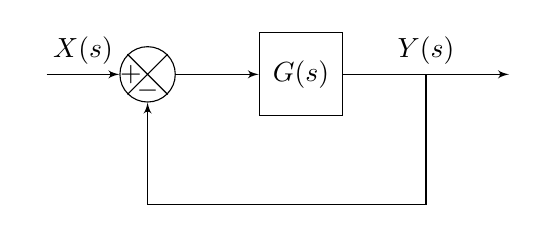
\begin{tikzpicture}
\sbEntree{E}
\sbComp{comp}{E}
\sbRelier[$X(s)$]{E}{comp}
\sbBloc[3]{B1}{$G(s)$}{comp}
\sbRelier{comp}{B1}
\sbSortie[6]{S}{B1}
\sbRelier[$Y(s)$]{B1}{S}
\sbRenvoi{B1-S}{comp}{}
\end{tikzpicture}
\end{document}